%-----------------------------------------------------------------------------------
%	PACKAGES AND OTHER DOCUMENT CONFIGURATIONS
%----------------------------------------------------------------------------------



\documentclass[11pt]{article}

\usepackage[top=2cm, bottom=3cm, left=2cm, right=2cm]{geometry}

\setlength{\parindent}{0in}

\newcommand{\Var}{\mathrm{Var}}

\newcommand{\Cov}{\mathrm{Cov}}

\newcommand{\plim}{\rightarrow_{p}}

\usepackage{amsmath, amsfonts}
\usepackage{graphicx}
\usepackage{pdfpages}
\usepackage{bm}
\usepackage{listings}

% Expectation symbol
\newcommand{\E}{\mathrm{E}}
\newcommand{\V}{\mathrm{V}}
\newcommand{\N}{\mathcal{N}}

\setcounter{section}{-1}

%----------------------------------------------------------------------------------
%	TITLE AND AUTHOR(S)
%----------------------------------------------------------------------------------

\title{Econ 675 Assignment 1} % The article title


\author{Nathan Mather} % The article author(s) 

\date{\today} % An optional date to appear under the author(s)

%----------------------------------------------------------------------------------
\begin{document}
	
%------------------------------------------------------------------------------
%	TABLE OF CONTENTS & LISTS OF FIGURES AND TABLES
%------------------------------------------------------------------------------
\maketitle % Print the title/author/date block

\setcounter{tocdepth}{2} % Set the depth of the table of contents to show sections and subsections only



\section{Empirical Exercises}


 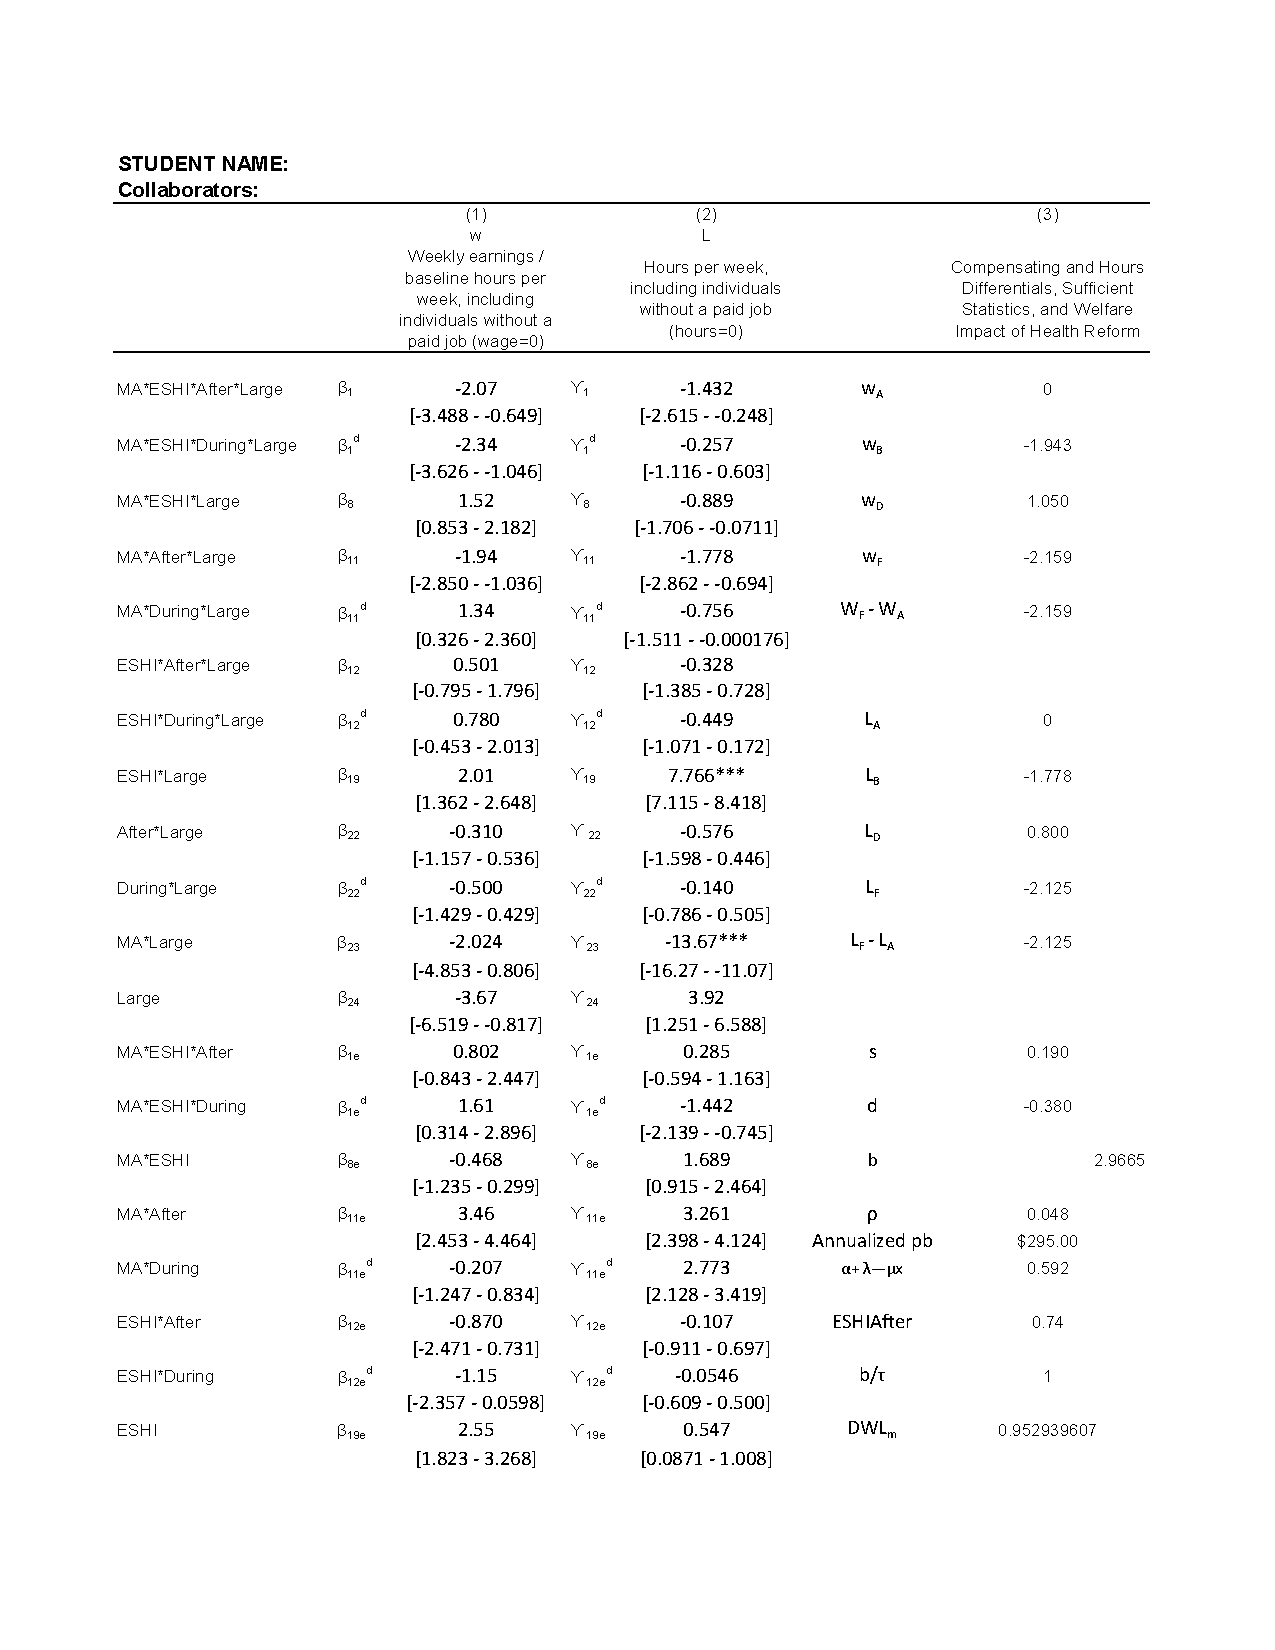
\includepdf[page=-]{Completed_sheet_1_5.pdf}


\section{Q1}

Because the reform also includes an individual mandate that everyone inside Massachusetts after the reform was treated in some way. so,$ V, X, V'',X''$ are all treated and the rest are controls. 


\section{Q2}

$\beta_1 = \{[(V-Y) - (X-Z)] - [(V'-Y') - (X'-Z')]\} - \{[(V'' - Y'') - (X''-Z'')] - [(V'''-Y''')-(X'''-Z''')]\}$

\section{Q3}

$\beta_1$ is the result of two stages of difference in difference. Start by doing four difference in differences of ESHI vs non-ESHI on the sub sections of Large and small MA firms and Large and small non-MA firms. These can be interpreted individually as th effect of reform one ESHI firms relative to non-ESHI firms in each category. After This, Take the difference in difference of these four sub estimate terms. Together we get the impact of reform on ESHI relative to non ESHI for large Massachusetts firms relative to small Massachusetts firms. 

\section{Q4}

First we can clearly see this is not correct by the equation given in the hint. What we want is the change in wages observed for individuals who switch from not having ESHI before the reform to having it after the reform, relative to individuals who have the same switch in ESHI status in other states. This is not $\beta_1$ . see above. 

\section{Q5}

By the hint we see that 
$$V = W_{MA, Large, ESHI, after} = \beta_1 + \beta_8 + \beta_{11} + \beta_{12} + \beta_{19} + \beta_{22} + \beta_{23} + (MA*Large) + \beta_{1e} + \beta_{8e} + \beta_{11e} + \beta_{12e} + \beta_{19e} + \beta_{22e} + \phi_{MA}$$ and 

$$ V' = W_{non-MA, Large, ESHI, after} = \beta_{12} + \beta_{19} + \beta_{22} + \beta_{23} + \beta_{12e} + \beta_{19e} + \beta_{22e} $$

This gives us 
$$ V-V' = \beta_1 + \beta_8 + \beta_{11} + (MA*Large) + \beta_{1e} + \beta_{8e} + \beta_{11e} + \phi_{MA}
$$

\section{Q6}

$$ Z = \beta_{23} + \phi_{MA} + (MA*Large)
$$
and 
$$Z' =  \beta_{23}$$

giving 
$$Z-Z' = \phi_{MA} + (MA*Large)$$

\section{Q7}

$$
x'' = \beta_{11e} + \beta_{22e} + \phi_{MA}
$$
and 
$$
Z'' =  \phi_{MA}
$$

so 
$$
X'' - Z'' =  \beta_{11e} + \beta_{22e}
$$

\section{Q8}

$$
X''' = \beta_{22e} 
$$

$$
z''' = 0
$$

so 
$$ X'''-Z''' = \beta_{22e}  $$

\section{Q9}

$$ W_f-W_A = (\beta_1 + \beta_8 + \beta_{11} + (MA*Large) + \beta_{1e} + \beta_{8e} + \beta_{11e} + \phi_{MA}) - (\phi_{MA} + (MA*Large)) - [(\beta_{11e} + \beta_{22e}) - \beta_{22e} ] $$

$$= \beta_1 + \beta_8 + \beta_{11} + \beta_{1e} + \beta_{8e}$$

\section{Q10}
This is the change in wages observed for individuals who switch from not having ESHI before the reform to hacing it after the reform, relative to individuals who have the same switch in ESHI status in other states. 

\section{Q11}
Because the most convincing identification comes from changes in ESHI status for a given individual induced by reform. The others rely on changes in ESHI status for a givin individual within the period either before or after the reform. The changes in ESHI status that identify these could be endogenous, even after including individual fixed effects, if individuals gain ESHI when they get a better job that includes health insurance. 

\section{Q12}
We expect it to be negative in theory because for a given individual at a given job if an employer is giving you health-care that is valuable they can compensate you less in actual wages and you will still want the job. However, it is usually the case that better jobs offer health care and low wage jobs don't. So, without individual fixed effects, it makes sense that we see jobs with healthcare having better pay. \\

Even with individual fixed effects the same idea can apply. An individual may get a better job that both pays more and includes health benefits. For example, if I was working at a fast food restaurant without healthcare, but I finish college and get a job as a research analysis with healthcare this would also lead to a positive compensating differential even with fixed effects. 

\section{Q13}
People above 64 are not in the data set at all. This makes since the elderly are required to use Medicare. \\

For the younger individuals I expect that they value healthcare less as they are, on average, healthier and also probably less risk averse. 

\section{Q14}
It goes down but is within the confidence interval. The reaffirms the idea that young people value the insurance less. 

\section{Q15}
 Increasing pb to \$3000 for the 25-64 population, $\rho$ increases from 0.048 to 0.486, and $DWL_m$ increases from 0.95 to 1.01. Thus, the higher penalty increases the deadweight loss of the mandate by 6\% 

\section{Q16}
The paper supports a mandate based reform as this leads to smaller dead-weight loss. In fact they find that $DWL_m/DWL_{\tau} = 0.077$ suggesting the mandate is much more efficient. 

\section{Q17}
The mandate-based reform is similar to the proposal under the ACA making it more applicable to the entire country. The differences in the actual penalty can be worked into the model for Massachusetts as is done on page 95.
\\ \\
However, there are some differences that could cause issues. Compliance may not be as high at the national level which could mean adverse selection remains high in the market for health insurance outside employers, making alternatives to ESHI less attractive. This would not effect the cost of healthcare to the employer, but it could effect the value of a dollar of ESHI relative to a dollar of wages because employees will value ESHI more if their outside option is more expensive. More adverse selection in the health insurance market outside of employment nationally could actually decrease reform-induced distortion. 

\section{Q18}
It would decrease distortion. 

\section{Q19}
It shouldn't change the interpretation weather or not people realize the tax is providing health-care. The tax and benefit are exogenous to the consumer regardless of if they are connected in the governments eyes.

\section{Q20}

This study allows us to consider an employer mandate on top of an existing individual mandate compared to taxes.

\section{Code}

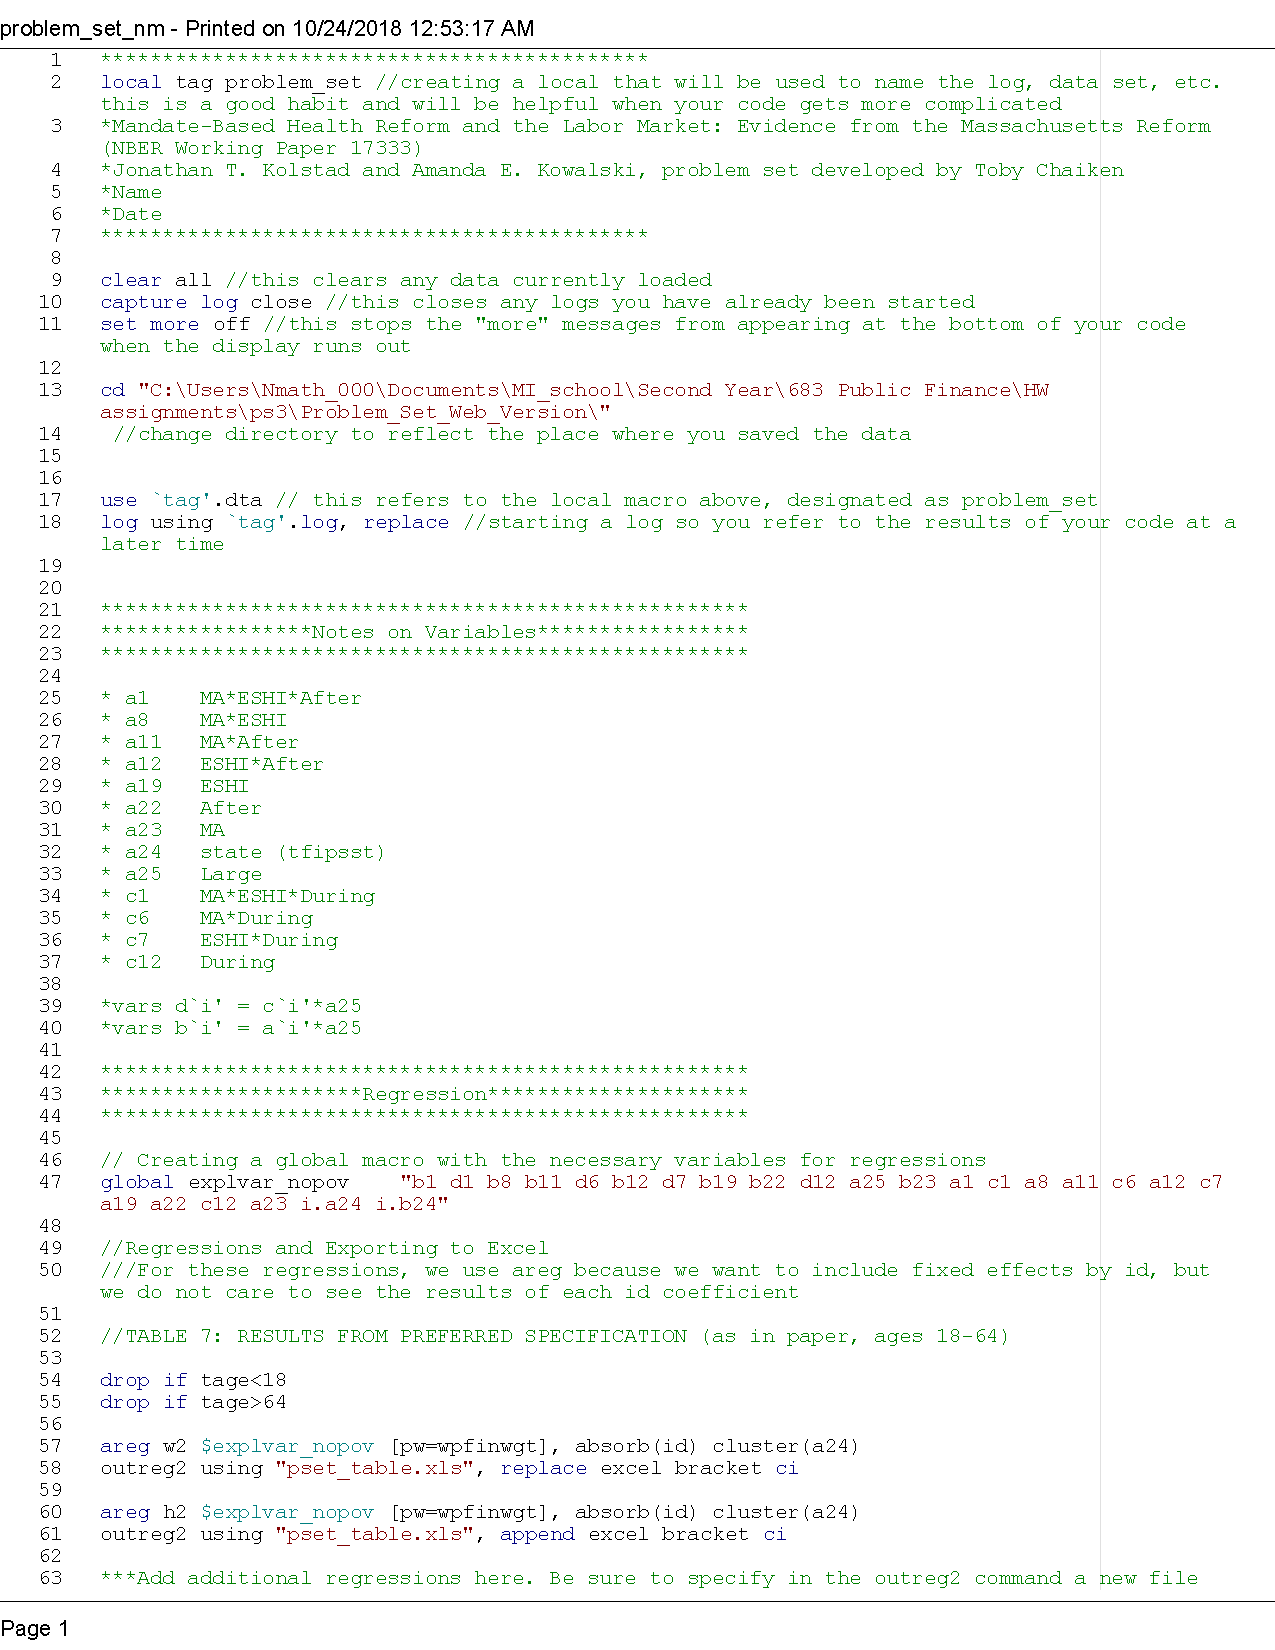
\includepdf[page=-]{code_683_ps3.pdf}



%------------------------------------------------
% end doc
%------------------------------------------------
\end{document}

